\chapter{Introduction}
\label{sec:intro}

Why does a person like a particular song? What are the inherent aspects of a song that pleases a person's musical taste? Is it the complexity of a song, the beat the song or just a particular melodic pattern ? More so if a person likes a song, can we predict if he/she will like a similar song? \\\\
Music has been created since the dawn of civilization and these questions have plagued mankind just as long. In response to this, man has created elaborate systems of formal study for music and classification techniques in almost every ethnic community since antiquity. Two notable examples are the western system of solfege and classical music theory and the Indian system of raagas. These elaborate systems are based on very simple fundamental building blocks of melody and harmony and simple rules that govern the interplay of these building blocks. However very complex pieces of music can be created with these simple rules depending on the skill and virtuosity of artists. Composers use these rules and concepts to create novel music for mass consumption. \\\\
In the modern era industry and academia have attempted to address the problem of music recommendation and music classification. The industry has predominantly favored approaches that look at user preferences and history. For example Amazon Music recommendation works on users shopping history. Pandora on the other hand hires an army of musicologists to ascertain how a song is similar to another song and creates software that leverages this adhoc generated data. These approaches are either expensive in the human labor needed or in the amount of data processed that is input from a large number of users. More recently, companies like Echo Nest has extensively extracted features from music sources and mined cultural information on the web but leave it at consumers how best to leverage the data. Hence symbolic MIR is not traditionally used in industry and music theory is an after thought. \\\\
Academia on the other hand attempts to solve very particular problems in MIR. Typical examples would be cover song detection, processing information via signal processing, audio feature extraction, optical music recognition etc. In most cases the applications are of a very specific domain and does not fully scale with bulk music data. Generic frameworks like the jMIR (which also happens to be a major inspiration for modulo7) suite for automatic music classification exists, which is meant to facilitate research in MIR with a machine learning focus. However academia is disconnected with industry and no full scale MIR engines can satisfy the scale of industry applications. \\\\
This work is attempt to bridge both communities. Modulo7 is a full stack deployment, providing both a server architecture and a sql like client to query based on music theory criteria.
\chapter{Software architecture}
The following sections present the software architecture of Modulo7.
\section{Server Side architecture}
\noindent Modulo7 is designed with the purpose of scalability. A block diagram of the components of the server side architecture is presented below :-
\begin{enumerate}
\item Source Converter : Converts music sources (e.g. music XML, midi etc) into modulo7's binary representation.
\item Music Theory Models : The model is a description of music theoretic criteria that can be applied on top of song. Examples would be melodic contour, tonal histogram etc. 
\item Distributed Storage Mechanism : The modulo7 internal representation is a conversion to create a song representation with all the meta data of the song (Key, Scale,  etc) along with the sequences of note events stored as lists. This representation is then serialized and stored in and Hadoop Distributed File System. This allows for fault tolerance and a distributed deployment of the input data.
\item Lyrics Indexer : A distributed index of songs lyrics. This acts as a base on which standard techniques for similarity analysis might be applied. Alternatively it can provide a framework on which custom models (e.g. semantic intent of the song, correlation between music theory models and lyrics might also be applied).  
\item Lyrics similarity models : A set of similarity models that can be applied to an index. 
\item Query Engine : An SQL like interface to a client that allows you to gather and ascertain useful information (based on music theoretic criteria). 
\end{enumerate}

\begin{figure}[t]
\centering
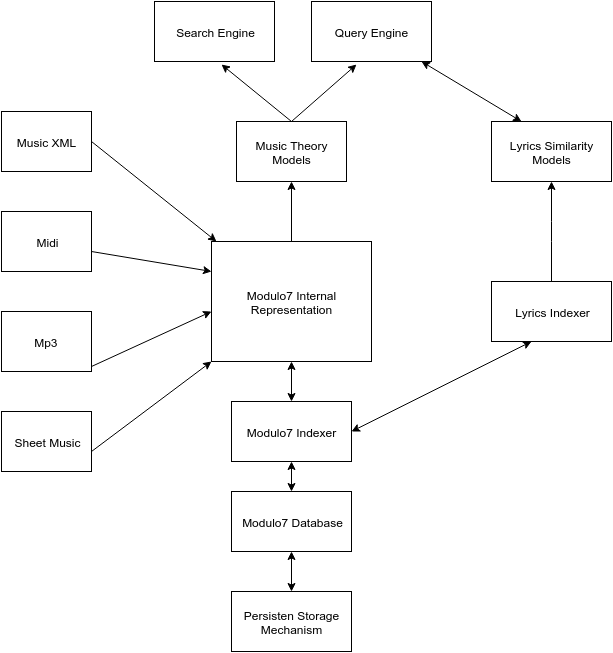
\includegraphics[width=\textwidth]{Modulo7Architecture.png}
\makeatletter
\let\@currsize\normalsize
\caption{Modulo7 architectural design}
\label{fig:figure}
\end{figure}
\section{Client architecture}
The server exposes a sql like interface as well as a consumable API. Some sample queries would be :-
\begin{enumerate}
\item select midi files from database where $melodic\_complexity > some threshold$
\item select * from database where $artist = led\_zepplin \ and \ harmonic\_movement > harmonic\_movement(stairway\_to\_heaven)$
\item select $ num\_voices \ from \ Database \ where \ songName = someSong.midi$ 
\end{enumerate}

An API will also be exposed to the client along a remote invocation procedure. The API would primarily target single sources for specifics. Some example API would be :-
\begin{enumerate}
\item int getNumVoices(String midiFilePath)
\item double melodicContourMovement(String pngSheetFilePath)
\item double compareAverageAttack(String musicXMLFile)
\end{enumerate}

This API can be consumed for specific song analysis. As design this API will not work on a bulk of files like its sql counterpart. 


\chapter{Progress Done}
The following points of progress have been successfully completed:-
\begin{enumerate}
\item Literature study on existing software related to Music Information Retrieval. Software exists which allow feature extraction {jMIR \cite{jMIR2010}.  - My primary inspiration}, Audio analysis and audio based Information Retrieval - {Essentia \cite{essentia}, marsyas \cite{marsyas}}, specialized music theoretic exploration of a song {Humdrum \cite{humdrum}}. None however attack the problem for MIR for scale. Also studied industry's approach on MIR, although companies don't publish all details. 
\item In the software architecture part : Completed the domain specific converters for Midi, Mp3 and Music XML along with the Modulo7 internal representation and its binarization. Need to start work on HDFS deployment.
\item Basic Lyrics indexer is implemented(including a tokenizer). Need to start work on lyrics similarity models. 
\item Identified non trivial amounts of datasets to begin testing on (e.g. the million song dataset for specific song features, JHU's Lester Levy Sheet music collection). I have started the process for acquisition of these datasets but working on these datasets would begin on October. 
\end{enumerate}
Points to consider and deliberate over:-
\begin{enumerate}
\item If certain meta data is not available, estimate that with existing algorithms (e.g if key of a song is not present, should the author include an estimation algorithm for it?).
\item Comparisons with other software. Other software try to address different problems so would have to compare different aspects of each software with Modulo7's components.
\item Criteria for evaluation (speed, accuracy of certain components with existing software etc). Need to figure out what other criteria are appropriate.
\item Investigate alternatively technologies for software design. (Need to be certain this is the best set of tools and design for this problem and this is the best possible architecture). 
\item How much breadth coverage is appropriate for the sql algebra space. Is numerical output the only statistics the author should consider or other qualitative aspects should also be a part of the design space?
\item Should the author attempt special problems already addressed in academia (e.g cover song detection) maybe with a different approach then existing literature?
\item Should the author work on a crawler and how should its scope be defined? While the author has worked on creating crawlers to mine domain specific sources, there might be copyright infringement on mining arbitrary sources. An alternative is to acquire data that is explicitly marked for research.
\item Should the author work on a "imprecise querying system" i.e. a search engine based on music theoretic criteria. This work would be extremely ambitious. 
\end{enumerate}